\documentclass[paper=a4, fontsize=11pt]{scrartcl}
%pre\'ambulo

\usepackage{lmodern} 
\usepackage[T1]{fontenc} 
\usepackage[spanish,es-tabla]{babel}
\usepackage[utf8]{inputenc} %%Tildes
\usepackage{mathtools}
\usepackage{wrapfig}  %Imagenes
\usepackage{enumitem}  %%Enumerado
\usepackage{hyperref}
\usepackage{eurosym}

\usepackage{url} % ,href} %para incluir URLs e hipervínculos dentro del texto (aunque hay que instalar href)
\usepackage{amsmath,amsfonts,amsthm} % Math packages
\usepackage{graphics,graphicx, float} %para incluir imágenes y colocarlas
\usepackage{subfig}

\usepackage{fancyhdr} % Custom headers and footers
\pagestyle{fancyplain} % Makes all pages in the document conform to the custom headers and footers
\fancyhead{} % No page header - if you want one, create it in the same way as the footers below
\fancyfoot[L]{} % Empty left footer
\fancyfoot[C]{} % Empty center footer
\fancyfoot[R]{\thepage} % Page numbering for right footer
\renewcommand{\headrulewidth}{0pt} % Remove header underlines
\renewcommand{\footrulewidth}{0pt} % Remove footer underlines
\setlength{\headheight}{13.6pt} % Customize the height of the header

\begin{document}

\title{Historia de la Robótica}
\author{Alicia Rodríguez Gómez}

\maketitle

\tableofcontents

\newpage

\section{Etapa Primeriza}




\subsection{Definición y Descripción de un Robot}


La realidad es que, lo que hoy día consideramos , no se asemeja a lo que en sus inicios se llamaba robot. Pero si que existen características generales que nos permiten llamar de la misma forma a los robot se empezaban a desarrollar desde la antigua Grecia y que naturalmente eran muy rudimentarios y a los robot que conocemos hoy día y que ayudan notablemente a facilitar la vida diaria a las personas.\\

Si nos limitamos a definiciones como pueden ser de la R.A.E. se dice que un robot es \textit{"Máquina o ingenio electrónico programable, capaz de manipular objetos y realizar operaciones antes reservadas solo a las personas."} Además de contar con las siguientes características:

\begin{itemize}
\item \textbf{Multifuncionalidad:} Capaz de llevar a cabo varias tareas.
\item \textbf{Programable:} Capaz de modificar su funcionalidad sin un excesivo costo.
\item \textbf{Alto Grado de Autonomía:} Capaz de ejecutar su tarea sin la intervención de un humano.
\end{itemize}

Pero nada más leer esta definición nos damos cuenta que esta definición no es válida ya que alrededor del año 400 a.C. no se podía hablar de máquinas programables y mucho menos electrónicas. La realidad es que el concepto de robots tal y como se conoce hoy en día, no se desarrolló hasta 1948 de la mano de George Devol. Más adelante se explicará con mayor profundidad la importancia de este en la historia de la robótica.

A modo de curiosidad, la palabra \textit{robot} tiene su origen en la obra teatral \textit{Robots Universales Rossum} dirigida por un dramaturgo checo que se estrenó en 1920. Es por tanto, que no fue hasta 1920 cuando comenzó a llamarse \textit{robot} a todo lo que vamos a describir en próximos aparatados.

\subsection{Orígenes de la Robótica (Griegos)}

Los primeros autómatas se desarrollaron en el Antiguo Egipcio. Como es natural estos no tienen nada que ver con lo que hoy se conoce como autómata, pero tenía bastante mérito para la época a la que pertenecen. Eso sí, se consideraban como tales ya que eran capaces de realizar determinadas tareas de forma autónoma. A continuación se van a mencionar los robot más relevantes de la época:\\

 \textbf{Arquitas de Tarento} en el año 400 a.C. diseñó \textit{"la paloma"}\ref{paloma}, ave mecánica que funcionaba con vapor. El mecanismo era muy rudimentario, debido a la época, y funcionaba de la siguiente manera; Se trataba de un objeto de madera con forma de paloma y se situaba colgada de una cuerda del techo. Esta contenía un pequeño depósito de agua, que se llevaba a ebullición mediante una llama situada en la parte inferior del depósito, y el vapor que se originaba se filtraba por unos pequeños orificios que le permitían al "\textit{robot}" simular el vuelo de la paloma.\\
 
\begin{figure}[H]
\begin{center}
  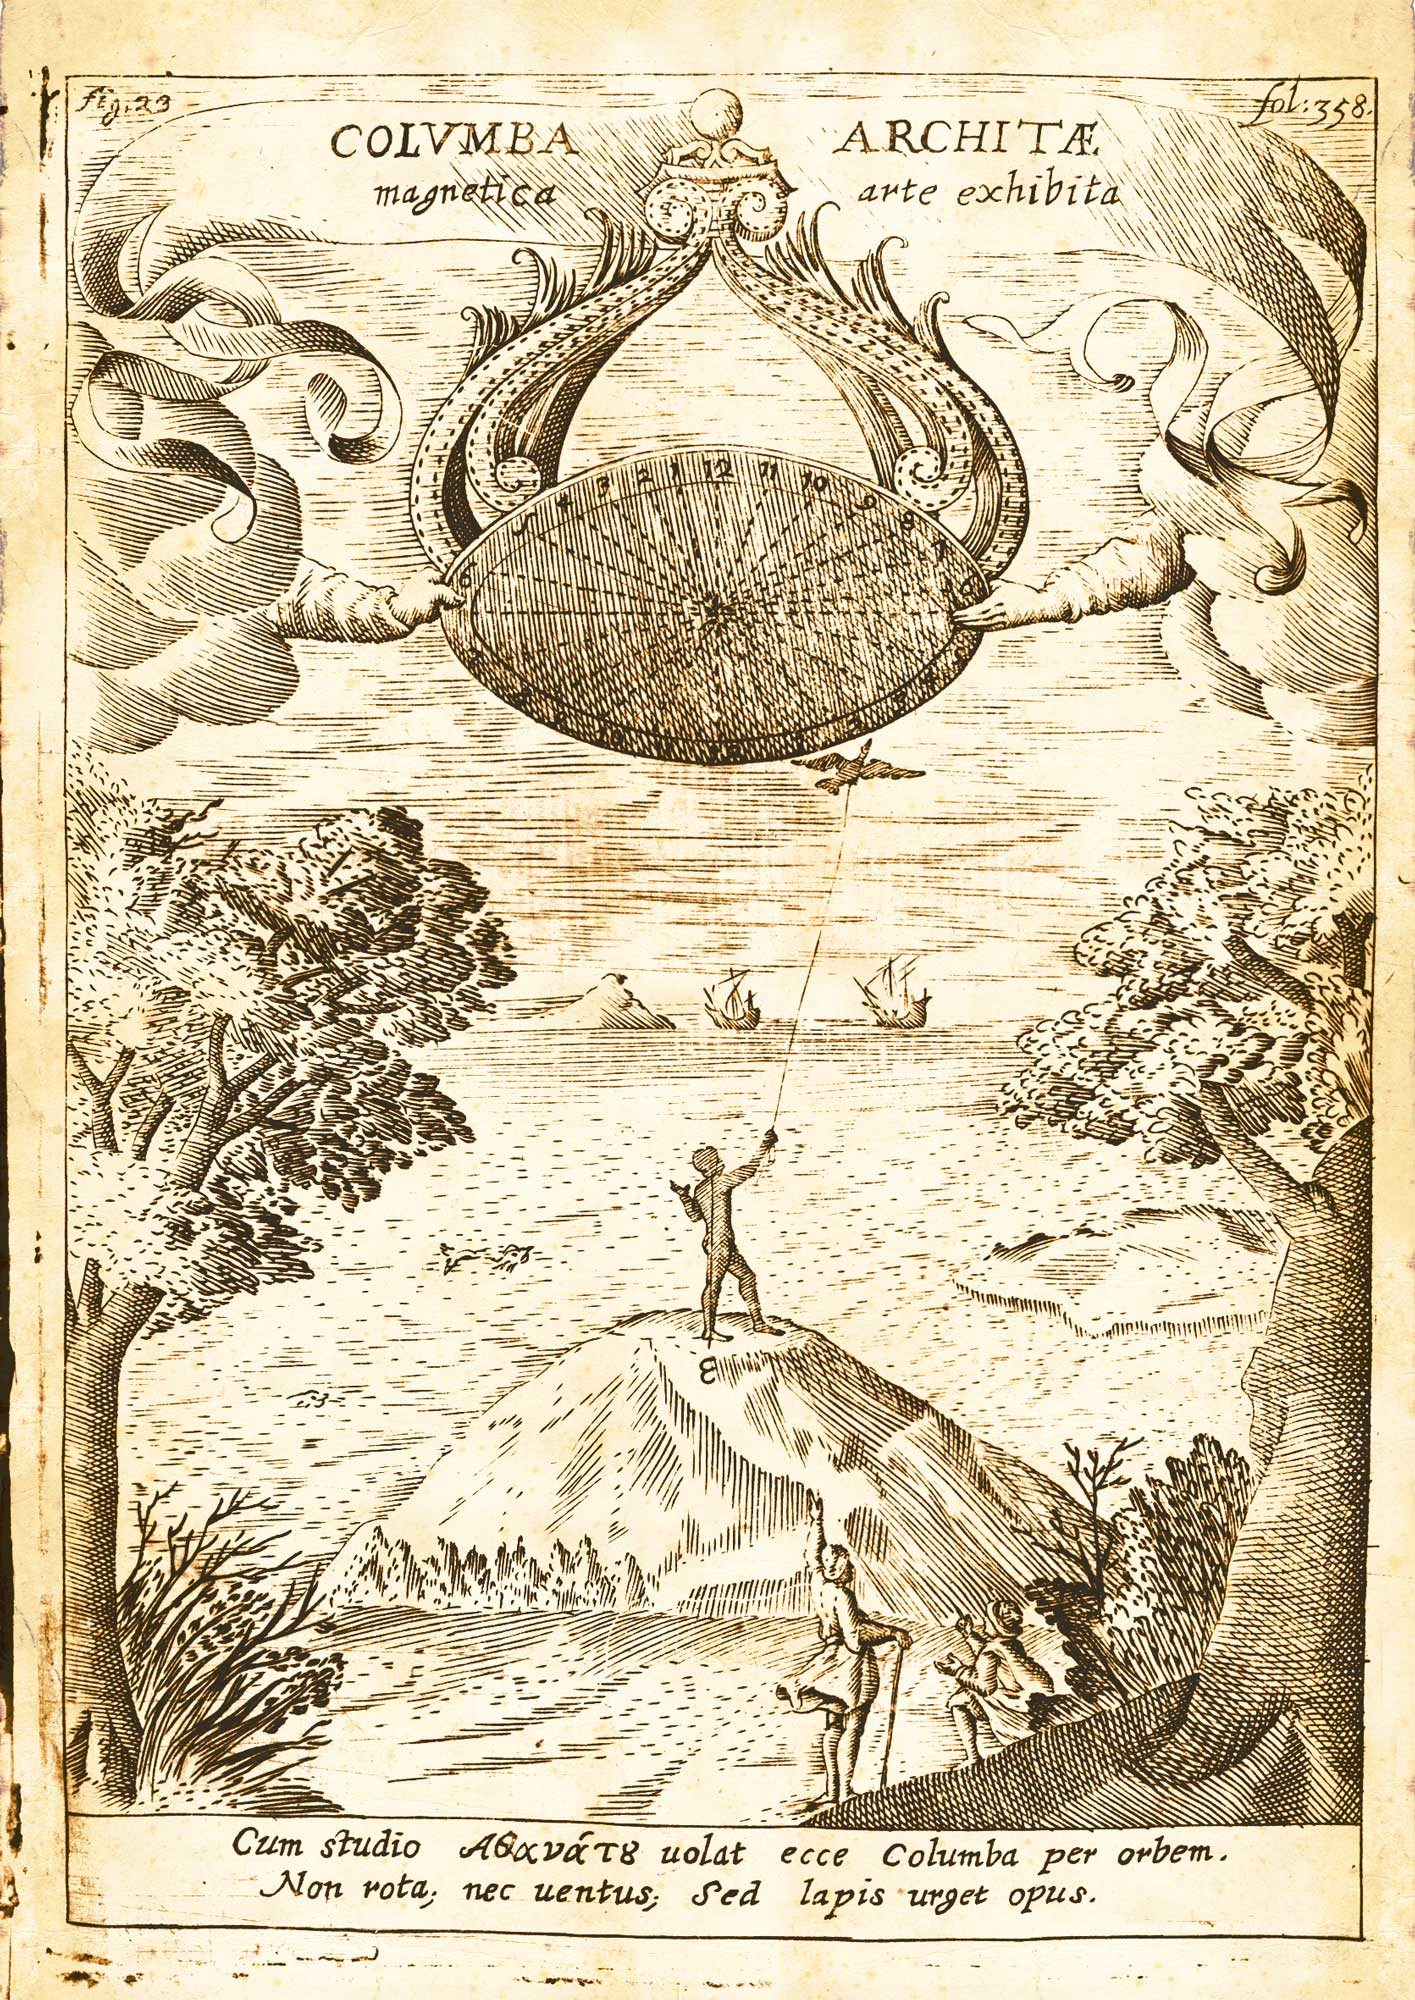
\includegraphics[width=0.5\textwidth]{imagenes/paloma.jpg}
  \caption{Paloma de Arquitas de Tarento}
  \label{paloma}
\end{center}
\end{figure}


Apolonio de Pérgamo, entre 262-190 a.C. , diseñó unos autómatas musicales que funcionaban impulsados por la fuerza del agua.\\


Ctesibio de Alejandría, en el año 300 a.C., también inventó autómatas musicales pero en este caso funcionaban por la impulsión de aire a través de diversos tubos. Pero su contribución más relevante fue el desarrollo del \textit{reloj de agua o clepsidra} que fue el más preciso de los relojes creados hasta la aparición del reloj de péndulo. Este mide el tiempo en función de lo que tarta en caer el agua de un recipiente a otro. Hasta ese momento, el tiempo se medía el tiempo a través de la observación del movimiento del sol, esto permitía medir el tiempo en cualquier momento del día. A continuación se muestra una imagen:\\

	
\begin{figure}[H]
\begin{center}
  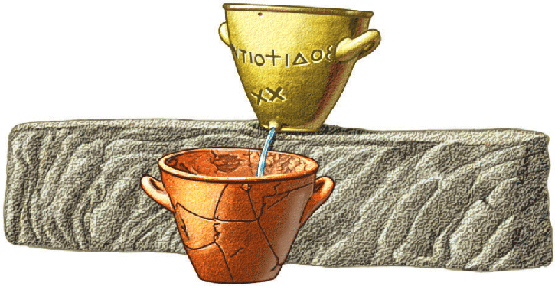
\includegraphics[width=0.5\textwidth]{imagenes/reloj.png}
  \caption{Reloj de Agua de Ctesibio de Alejandría}
  \label{reloj}
\end{center}
\end{figure}



Filón de Bizancio inventa en el año 200 a. C.,\\

Heron de Alejandría: desarrolló numerosos inventos de los que dejó constancia escrita en Neumática –un tratado sobre hidráulica– y Los autómatas, seguramente el primer libro sobre robótica de la historia. Entre otros artilugios pasmosamente modernos, Herón de Alejandría describe pájaros que volaban y gorjeaban, y diversos modelos de estatuas que imitaban el comportamiento humano o, más exactamente, el de los esclavos, pues la mayoría se construyeron para servir vino y comida durante los banquetes. También, un dispositivo que abría y cerraba automáticamente las puertas de los templos; la primera máquina térmica de la historia –denominada eolípila–; y la ahora conocida como Fuente de Herón, un artilugio para el aseo personal de quienes acudían a las ceremonias religiosas que funcionaba introduciendo una moneda.\\


En año 335 d. C., Hsieh Fec

En el 770 d. C., Yang Wu-Lien 

El príncipe Kaya construye en el año 840

En el 890, Han Chih Ho

En el año 1050 el príncipe hindú Bhoja

En el siglo XII Al-Jazari (o Al-Djazari)

El Gallo de Estrasburgo, el robot más antiguo que se conserva en la actualidad, funcionó desde 1352 hasta 1789.

En España, el Papamoscas de la catedral de Burgos, construido en el siglo XVI, consiste en un hombre mecánico que se mueve con los cambios horarios y funciona aún hoy día

Los autómatas más famosos del medioevo son el hombre de hierro de Alberto Magno (1204-1282) o la cabeza parlante de Roger Bacon (1214-1294)





 

\subsection{Sistemas Mecánicos Simples}

Cuando nos referimos a Sistemas Mecánicos Simples\ref{sms} se hace referencia a aquellos formados principalmente por componentes, dispositivos o elementos que tienen como función transformar o transmitir el movimiento desde las fuentes que los generan al transforman distintos tipos de energía.

A continuación se describen los principales Sistemas Mecánicos Simples:

\begin{itemize}

\item \textbf{La Rueda:} Pieza mecánica circular que rota alrededor de un eje.

\begin{itemize}
\item El Rodillo: Se trata de un cilindro con un diámetro ancho y con una destacada longitud, que al igual que lo hace la rueda, gira alrededor de un eje.

\item Tren de Rodadura
\item Rueda Dentada: Se trata de una rueda cuyo perímetro está totalmente cubierto de dientes. Su ventaja recae en proporcionar movimiento circular mediante el contacto de los dientes entre dos ruedas.

\item Polea Fija: Se trata de una polea en el que la polea se encuentra fija en la parte superior.

\item Polea Móvil: Se trata de una polea conectada a una cuerda en cuyos extremos está, por un lado, anclada a un punto fijo y en otro a un extremo móvil.

\item Polipasto: Conjunto de poleas en la cual una queda fija y la otra tiene movilidad.


\end{itemize}

\item \textbf{La Palanca} 

\begin{itemize}
\item Palanca de Primer Grado: Se trata de una palanca donde el punto de apoyo se sitúa entre la Potencia y la Resistencia. Un ejemplo claro de este tipo de palanca podría ser unas tijeras o una balanza.

\item Palanca de Segundo Grado: Se trata de una palanca en la cual la Resistencia se sitúa entre el punto de apoyo y la fuerza. Un ejemplo de este tipo de palanca podría ser un cascanueces o una carretilla de obra.

\item Palanca de Tercer Grado: Se trata de una palanca en la cual la fuerza se sitúa entre la resistencia y el punto de apoyo. Un ejemplo de este tipo de palanca podría ser un martillo o una caña de pescar.

\end{itemize}

\item \textbf{Plano Inclinado}

\begin{itemize}
\item La Rampa: Superficie plana que forma un ángulo agudo con la superficie.

\item Cuña: Se trata de un prisma triangular que actúa como un plano inclinado móvil.

\item Sistema Tornillo-Tuerca: Sistema en el que un tornillo rota en el interior de una tuerca. Se utiliza para unir de forma no permanente dos elemento.

\item Tirafondo: Tipo de tornillo que tiene una cabeza diseñada para ejercer el giro en esta mediante la ayuda de una herramienta.

\end{itemize}

\end{itemize}

\subsection{Leonardo da Vinci}

Leonardo da Vinci (1452-1519) construyó para el rey Luis XII de Francia un León Mecánico, que se abría el pecho con la garra y mostraba el escudo de armas real. En 1495 ya había diseñado uno de los primeros autómatas humanoides del mundo occidental: un caballero con armadura, capaz de incorporarse, agitar los brazos, mover la cabeza (tenía un cuello flexible) y abrir y cerrar la mandíbula. Estas máquinas se relacionan con el canon anatómico del hombre vitruviano y sus claves matemáticas. Alrededor del año 1500 diseñó también una máquina de cálculo, predecesora de la que Blaise Pascal inventaría más de un siglo después por lo que el genio italiano proyectó la robótica desde el punto de vista formal y computacional

\subsection{Máquina Calculadora de Pascal}

\subsection{Autómatas en miniatura del siglo XVIII}

\subsection{Robótica y Maquinaria en los talleres textiles}

\subsection{Hasta el siglo XIX}

\subsection{Isaac Asimov y las reglas de la robótica}

\subsection{Tortugas autónomas de Walter}

\subsection{El brazo robótico teleoperado de Goertz}

\subsection{Autónoma Universal de George Devol}

\textbf{George Devol} es conocido como el creador del primer robot industrial además de cofundador de la primera empresa robótica de la historia.

\subsection{Sputnik}

El programa \textbf{Sputnik} se trataba de una serie de misiones espaciales ejecutadas por la antigua Unión Soviética a finales de los años 50 y principios de los 60 del siglo pasado. El objetivo de este programa era probar la viabilidad de los satélites artificiales alrededor de la órbita de nuestro planeta.
Como curiosidad, señalar que el origen de la palabra \textit{Sputnik} proviene del ruso y significa \textit{satélite} o \textit{compañero de viaje}.
Durante este programa se lanzaron al espacio hasta 10 satélites diferentes. Seguidamente se describirán cada uno de ellos y el impacto que esto tuvo.\\


\textbf{Sputnik 1}\ref{s1} fue el primer satélite artificial de la historia el cual fue lanzado el 4 de Octubre de 1957. La importancia de este satélite recae en que fue el primer intento sin fallo de poner a orbitar alrededor de nuestro planeta un satélite artificial. Fue lanzado con el lanzador R-7 y este se encargó de analizar señales de radio que utilizaba para conocer la cantidad de electrones en la ionosfera. Estuvo en actividad durante 92 días y en la actualidad se puede visitar en la oficina neoyorkina de las Naciones Unidad.\\ 

\begin{figure}[H]
\begin{center}
  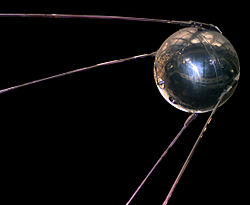
\includegraphics[width=0.5\textwidth]{imagenes/s1.jpg}
  \caption{Sputnik 1}
  \label{s1}
\end{center}
\end{figure}

Más tarde, se lanzó el \textbf{Sputnik 2}\ref{s2} el 3 de Noviembre de 1957. A diferencia del \textit{Sputnik 1}, este portaba un ser vivo en su interior. Aquí viajó la conocida \textit{Perra Laika}, y el objetivo de este lanzamiento era comprobar el efecto que causaba el medio espacial en un ser vivo. Regresó a La Tierra tras 162 días de actividad y en aquel momento de publicó que \textit{Laika} murió al regreso a nuestro planeta. Sin embargo, en 2002 fuentes rusas declararon que el animal había muerto al poco tiempo de ser lanzada a causa del estrés y el sobrecalentamiento del satélite.\\

\begin{figure}[H]
\begin{center}
  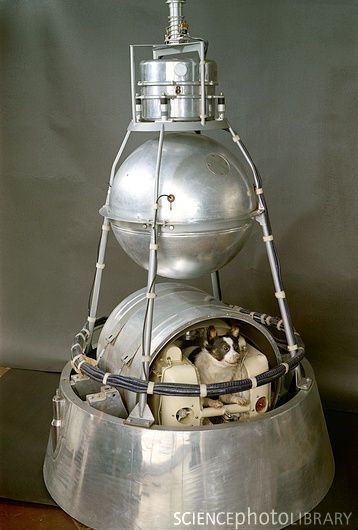
\includegraphics[width=0.3\textwidth]{imagenes/s2.jpg}
  \caption{Sputnik 2 con Laika en su interior}
  \label{s2}
\end{center}
\end{figure}

Fue el 3 de Febrero de 1958 cuando se intento lanzar el siguiente satélite, \textbf{Sputnik 3}. Esto quedó en un solo intento ya que fue fallido. Pero más tarde, se consiguió volver a lanzar esta vez ya correctamente. A pesar de que el sistema de grabación falló, transportó instrumentos para explorar la atmósfera superior y el espacio próximo.\\

\textbf{Sputnik 4} que fue lanzado el 15 de Mayo de 1960, fue el primer prototipo de nave espacial lanzada desde nuestro planeta y llevaba a bordo un maniquí de un hombre, un sistema de televisión y una cabina de soporte biológico. Pero un fallo en el sistema de guía la reubicó en una órbita más alta a la terrestre. Regresó el 5 de Septiembre de 1962, pero nada más tomar contacto con la atmósfera terrestre se desintegró. Algunas de sus piezas fueron encontradas al norte de los Estados Unidos, en Wisconsin.\\

Más tarde, el \textbf{Sputnik 5} se lanzó el 19 de agosto de 1960 y esta llevaba a bordo a los perros \textit{Belka} y \textit{Strelka} además de 40 ratones y numerosas plantas. La nave solamente permaneció en el espacio un día y todos los seres vivos regresaron con vida.\\

\textbf{Sputnik 6} fue enviado al espacio el 1 de Diciembre de 1960 con los perros \textit{Pchelka} y \textit{Mushka} junto a una serie de insectos, animales y plantas, y la cápsula no se consiguió recuperar. \\

Más tarde, el 4 de Febrero de 1961, \textbf{Sputnik 7} fue el primer intento de exploración de Venus. Sin embargo, el sistema de ignición tuvo un fallo y la sonda regresó a la órbita terrestre en lugar de tomar dirección a Venus.\\

Seguidamente, \textbf{Sputnik 8} se envió el 12 de Febrero de 1961 que transportaba la sonda Verena 1. Esta fue la primera nave espacial lanzada para sobrevolar el planeta Venus.\\

\textbf{Sputnik 9} fue una de las pruebas que tenían como finalidad precursar los vuelos espaciales tripulados por humanos. Este completó un giro completo alrededor de nuestro planeta y volvió sin ningún problema lo que supuso un gran éxito.\\

Finalmente el \textbf{Sputnik 10}, al igual que el \textbf{Sputnik 9}, se trataba de una serie de pruebas con naves espaciales diseñadas para tripulación humana. Este portaba un perro, un astronauta ficticio y un sistema de televisión. Al igual que el anterior, se recuperó con éxito.

\begin{figure}[H]
\begin{center}
  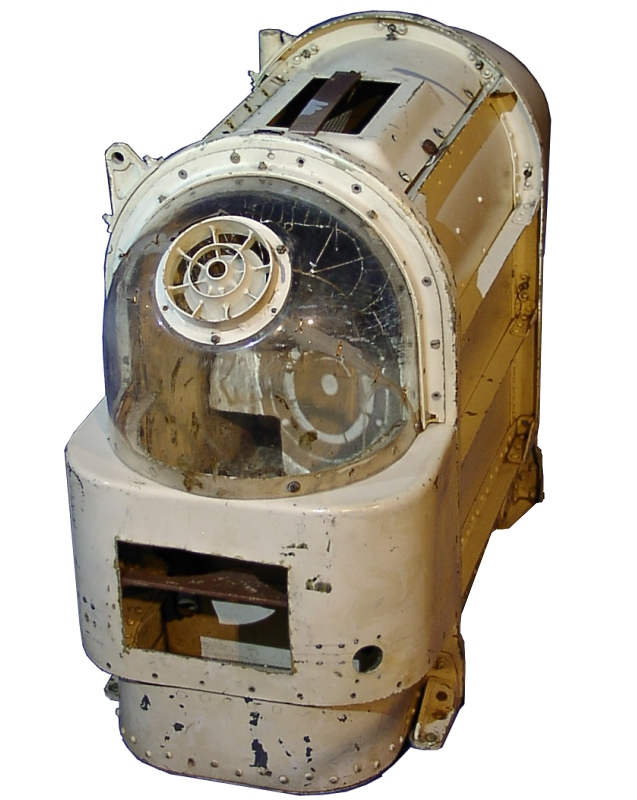
\includegraphics[width=0.3\textwidth]{imagenes/s10.jpg}
  \caption{Sputnik 10}
  \label{s2}
\end{center}
\end{figure}





\subsection{Robots Industriales de Generals Motors}




\section{Bibliografía}







\end{document}